\documentclass[12pt]{article}

\usepackage{hyperref}
\usepackage[utf8x]{inputenc}
\usepackage{graphicx,url}
\usepackage{longtable,tabu}
\usepackage[brazil]{babel}
\usepackage{natbib} % Tidies up citation numbers.
\usepackage{url} % Provides better formatting of URLs.
\usepackage{hyperref}
\usepackage{geometry}
\geometry{a4paper,total={150mm,237mm},left=30mm,top=35mm}
\pagestyle{plain}
\pagenumbering{arabic}
%\renewcommand{\baselinestretch}{1.5}

\sloppy

\begin{document}
	\title{O Design Fiction como ferramenta para uma computação ética}

	\author{André Carvalho Marques}

	\renewcommand{\tablename}{Quadro}

	\newcommand{\address}{{
			\begin{center}
				\footnotesize
				Universidade de Brasília - Instituto de Ciências Exatas\\  Departamento de Ciência da Computação - CIC 116726 - Informática e Sociedade \\
				2017.2 - Turma A - Professor Jorge Henrique Cabral Fernandes\\ Prédio CIC/EST - Campus Universitário Darcy Ribeiro \\Asa Norte 70919-970 Brasília, DF\\
				\href{mailto:andre.marques@aluno.unb.br}{andre.marques@aluno.unb.br}
			\end{center}
	}}

	\maketitle
	\address

	\begin{abstract}
		Nosso mundo está constantemente se alterando, e com essas alterações vem alguns problemas éticos, como por exemplo, um robô com uma inteligência artificial suficientemente boa para se passar por humano deve ter os mesmos direitos de um humano? O trabalho Operationalizing Design Fiction for Ethical Computing fornece alguns pontos interessantes a respeito da análise da ética em universos futuros, a partir do filme Frank e o Robô é criada toda uma análise ética e um documentário chamado de Care for a Robot. Em Care for a Robot temos a oportunidade de conhecer as opiniões de pessoas fictícias deste universo. Estes personagens foram criadas com o auxílio de pessoas que foram entrevistadas após assistirem pedaços selecionados do filme Frank e o Robô e receberem a explicação de determinados termos relacionados ao Design Fiction, houve então uma breve discussão de no máximo 30 minutos da qual foram retirados trechos de respostas para serem apresentadas a nós. O objetivo do trabalho não é tanto a discussão do filme em si quanto é a discussão de: seria o Design Fiction uma ferramenta interessante para explorar estes dilemas éticos?

		\textbf{Palavras-chave:} \textit{Informática e Sociedade. UnB. Design Fiction.}
	\end{abstract}

	\section{Introdução}
	\par É evidente que a sociedade na qual vivemos passou por mudanças profundas e significativas desde o início do século passado. Hoje temos preocupações muito diferentes das que já tivemos, estas preocupações são em parte graças aos avanços tecnológicos da humanidade. Algumas destas preocupações novas seriam por exemplo a vigilância do indivíduo pelo Estado em meios digitais de forma indiscriminada, invasões de sistemas que podem causar grandes perdas financeiras e etc. mas por vezes nos prendemos nos problemas do presente e não consideramos questões que possam surgir no futuro, o que acaba causando o problema da ética não ser capaz de acompanhar a tecnologia.
	\par
	Este artigo se baseia no artigo \cite{lindley_operationalising_2016} em que se discute a humanidade presente em robôs que possuam uma inteligencia avançada o suficiente para ser considerada humana no artigo é utilizado como base para esta discussão o filme \textit{Frank o Robô} e um mini documentário chamado de  \textit{Care for a Robot}. No documentário conhecemos vários personagens que nos apresentam suas próprias visões de mundo de acordo com a diegética do universo criado. Com isso podemos ter uma visão valiosa de como a humanidade como um todo poderá vir a ver questões iguais ou parecidas. Sendo assim tem-se como objetivo deste trabalho apresentar o \textit{Design Fiction} como uma ferramenta valiosa no que tange o comportamento da sociedade em vista de tecnologias que atualmente seriam consideradas impossíveis.


	\section{\label{organizacao:artigo}Organização, formatação e entrega do artigo}

	O artigo deve conter uma introdução, um desenvolvimento e uma conclusão, além de referências.
	O artigo deve ser entregue de forma digital, preparado para impressão em papel no formato A4, com tamanho de 12 a 20 páginas, incluídas as referências.
	O artigo deve ser preparado com o processador de texto \LaTeX.
	Para os que não tem experiência com o uso do \LaTeX, recomenda-se fortemente o uso da plataforma \href{http://www.overleaf.com}{Overleaf}, que facilita a edição de textos \textit{online}.

	O trabalho deve ser entregue em um arquivo digital em formato ZIP, com o nome $<$NomeCompletoDoAluno-Matricula$>$.zip (Ex: JorgeHCFernandes-1012606.zip), contendo duas partes:
	\begin{itemize}
		\item Artigo em formato PDF;
		\item Diretório contendo os textos, figuras originais, arquivos .bib e outros, no formato de fonte \LaTeX, que permitam compilar e gerar o PDF.
	\end{itemize}

	O documento em PDF será usado para fins de atribuição de pontuação.
	A entrega em formato de fonte \LaTeX\ permitirá que o texto possa futuramente sofrer edições para constituição de um livro para referências.
	Nesse último caso, o(a) autor(a) será consultado(a) sobre interesse em publicação.

	O texto deve ser desenvolvido em coluna simples, e o tamanho das margens deve ser: superior = 3,5 cm; inferior = 2,5 cm; esquerda = 3,0 cm; direita = 3,0 cm.
	O espaçamento deve ser: 1,5 entre linhas; sem espaçamento entre parágrafos.

	Não devem existir cabeçalhos nem rodapés, com exceção da numeração de página.
	Todos esses parâmetros de formatação são automaticamente ajustados pelo uso do editor \LaTeX e do template fornecido.

	\section{\label{secoes:texto}Seções do texto}

	O texto deve possuir pelo menos seis distintas seções:
	\begin{description}
		\item [Introdução] Na qual o autor deve motivar a abertura do debate, por meio de apresentação de um resumo do artigo base, e de uma crítica ao debate incitado pelo artigo.
		\item [Metodologia] Na qual o autor deve citar e explicar a proposta de \citet{jones_doing_2016}, de desenvolver um debate sobre ética para estudantes de informática com base em um arcabouço baseado em seis momentos, que também será utilizado nesse artigo. Portanto, a definição da metodologia de desenvolvimento do artigo é baseada na proposta de \citet{jones_doing_2016}.
		\item [Dilemas éticos] Com base na proposta de \citet{jones_doing_2016}, o artigo deve fazer uma citação e análise dos principais dilemas éticos que o autor crê estão em jogo no debate aberto pelo artigo apresentado na introdução. O texto deve citar exatamente quais são os valores ou conceitos éticos que poderão estar sendo conflitados, e oferecer referências bibliográficas para fontes de informação que definem de forma mais precisa quais são esses valores.
		\item [Análise Tecnológica] Nesta seção o autor deve analisar as principais tecnologias de informação e comunicação relacionadas com o debate incitado pelo artigo motivador. Para fazer tal análise, é necessário apresentar referências a empresas, marcas ou organizações humanas envolvidas com essas tecnologias. Mais detalhes são apresentados na subseção \ref{tecno}.
		\item [Momento ético] Partindo de um ou mais casos específicos de desenho, implantação e uso de uma tecnologia real ou especulativa, o autor deve fazer uma declaração explícita dos valores e princípios que poderão estar em jogo nesses casos. Devem ser feitas referências a autores que definem o que são esse valores. Apenas apresente e justifique o que poderá estar em jogo.
		\item [Momento legal ou jurídico] Na qual o autor deve indicar quais são as distintas áreas de jurisdição legal na qual se encontram os contextos de desenho, implantação e uso das tecnologias analisadas.
		Mais detalhes na subseção \ref{legal}.
		\item [Momento do praticante]
		Partindo das considerações prévias sobre as questões sociais, éticas e legais envolvidas com o \textit{design}, implantação e uso de tecnologias específicas, o autor deve identificar uma ou mais profissões ou atividades profissionais envolvidas, e indicar quais códigos de conduta seriam aplicáveis.

		Devem ser abordados aspectos como responsabilidades, conduta moral e ética, ligados à profissão.

		Deve ser considerada uma ampla gama de profissões, tais como gestores, usuários, pesquisadores, engenheiros, programadores, designers, analistas de sistema, empregados públicos, ou organizações tais como empresas privadas que desenvolvem sítios, jogos, etc.
		\item [Conclusões] O texto deve apresentar conclusões, encaminhamentos, sínteses e abertura de outras questões, que permitam solucionar os dilemas apresentados.

	\end{description}

	\subsection{\label{tecno}Análise contextualizada das tecnologias de informação e comunicação}

	O texto precisa citar tecnologias, marcas, empresas e pessoas que tem afinidade com os problemas e dilemas levantados pelo artigo.

	Para que seja feita uma análise contextualizada das tecnologias de informação e comunicação é necessário que o autor descreva, para as tecnologias citadas, quais ele crê que sejam os distintos contextos sociais envolvidos no projeto (\textit{design}), implantação (\textit{deployment}) e uso das tecnologias específicas. Em outras palavras, uma tecnologia precisa ser analisada sobre esses três prismas distintos, para que se entenda as questões éticas por trás dela.

	Devem ser buscadas informações que permitam serem discutidos em quais contextos sociais, históricos, políticos, econômicos etc, ocorreram o projeto, a implantação e o uso das tecnologias específicas.

	Note que tecnologia usualmente tem nome, marca, está vinculada a uma ou mais empresas etc. Tecnologia usualmente também envolve patentes e pesquisas científicas e tecnológicas, bem como o uso de protótipos. É também possível tratar de tecnologias que ainda não foram efetivadas para uso na sociedade. Nesse caso, o autor terá que desenvolver um artigo especulativo, apresentando um cenário ficcional.

	Para essas tecnologias o autor deve abordar os principais fatos ou especulações (o que? onde? como? quem? quando? por que?) relacionadas ao design, implantação e uso da tecnologia, bem como quem seriam as principais pessoas ou empresas envolvidas, interessadas e potencialmente impactadas (\textit{stakeholders}) pela tecnologia.

	Observe que no aprofundamento do trabalho final o autor deverá também, com base em algumas das orientações providas por \citet{jones_doing_2016}:
	\begin{itemize}
		\item  Mostrar quais são os principais direcionadores econômicos (oferta e demanda, compra e venda etc) e políticos (grupos de interesse, discussões e conflitos) presentes e relacionados ao design, implantação e (ou) uso da tecnologia.

		\item  Tratar de quais valores (princípios da ética e moral) estão embutidos nas características específicas, relevantes e evidentes dessas tecnologias. Por exemplo, quais os valores por trás do \textit{marketing} e da propaganda usadas para promoção das tecnologias? Por exemplo, a competitividade, o estilo de vida, a saúde, a justiça, o desenvolvimento econômico, a sustentabilidade, a empatia etc, estão presentes no design, implantação e (ou) uso da tecnologia específica?

		\item  Embasar sua análise ou especulação em fatos, com referências para fontes de informação, como jornais, sítios web, revistas, registros administrativos, relatórios etc.
	\end{itemize}

	Na conclusão da introdução, o autor deve apresentar um sumário dos principais principais dilemas éticos que estão em jogo no debate aberto pelo artigo, citando-os explicitamente.

	\subsection{\label{legal}Momento Jurídico ou Legal}
	O autor deve explorar brevemente quais leis e arcabouços regulatórios se aplica ou poderiam se aplicar às tecnologias em foco.

	Devem ser apresentadas referências ou nomes de leis, e outras fontes de informação sobre legislação.

	O autor deve sugerir ou aventar quais seriam os potenciais interesses políticos e econômicos por trás de uma ou mais das leis indicadas.

	No trabalho final, o autor também deve discutir sobre a legitimidade ética por trás das leis citadas.

	No caso de falta de legislação, o autor deve especular sobre quais legislações poderiam ser aplicáveis, de modo a auxiliar na solução de potenciais conflitos que surgiram ou poderiam surgir.

	\subsection{\label{conteudos}Emprego dos conteúdos e conceitos já abordados na disciplina}

	Onde pertinente, o artigo deve demonstrar que o autor sabe lançar mão dos conteúdos e operar sobre os conceitos abordados nos textos usados nas fases anteriores da disciplina.

	\section{\label{rubrica}Rubrica de avaliação do artigo}
	A avaliação do artigo obedecerá a uma rubrica de avaliação composta por 7 aspectos, totalizando 70 pontos. Esses aspectos são apresentados a seguir.

	\subsection{Adota formato de artigo científico}
	Entre 0 a 10 pontos serão atribuídos ao artigo pelo avaliador conforme a resposta à seguinte questão: O texto está no formato de um relatório ou artigo científico?

	\subsection{Compreende os artigos originais}

	Entre 0 a 10 pontos serão atribuídos ao artigo pelo avaliador conforme resposta à seguinte questão: O texto demonstra que o autor conseguiu entender do que tratam os artigos usado como base para sua argumentação, que são o artigo inicial, combinado com o texto de \citet{jones_teaching_2016}?

	\subsection{Dilemas e momentos éticos}
	Entre 0 a 10 pontos serão atribuídos ao artigo pelo avaliador conforme resposta à seguinte questão: O texto demonstra que o autor conseguiu operar sobre conceitos e valores éticos e morais?

	\subsection{Análise Tecnológica}
	Entre 0 a 15 pontos serão atribuídos ao artigo pelo avaliador conforme resposta à seguinte questão: O texto consegue demonstra que o autor buscou analisar de forma aprofundada as tecnologias por ele investigadas, no que se refere aos aspectos de desenho, implantação e uso? Foram referenciados os argumentos, com fontes de boa qualidade?

	\subsection{Análise legal ou jurídica}
	Entre 0 a 10 pontos serão atribuídos ao artigo pelo avaliador conforme resposta à seguinte questão: O texto demonstra que o autor buscou informações relevantes no campo jurídico ou legal, para embasar sua análise? os argumentos apresentados são de boa qualidade e de fácil compreensão?

	\subsection{Utilização dos outros conteúdos abordados na disciplina}
	Entre 0 a 5 pontos serão atribuídos ao artigo pelo avaliador conforme resposta à seguinte questão: O texto demonstra que o autor se apropriou de outros conceitos abordados na disciplina, como a discussão sobre a Estratégia Brasileira da Transformação Digital, entre outros?

	\subsection{Conclusões}
	Entre 0 a 10 pontos serão atribuídos ao artigo pelo avaliador conforme resposta à seguinte questão: O texto apresenta conclusões ou encaminhamentos para a solução dos dilemas e problemas encontrados e mapeados?

	\section{\label{mais:orientacoes}Mais orientações sobre organização do artigo}

	\subsection{Tabelas e quadros}

	O artigo deve lançar mão de tabelas e quadros, para organizar a informação apresentada. Todos esses elementos devem estar centralizados, e apresentar um título também centralizado. Usa-se ainda uma numeração sequencial para a apresentação dos mesmos (Quadro 1, Quadro 2, Tabela 1, Tabela 2 etc). Todas as tabelas e quadros devem ser textualmente apresentadas.

	\subsection{Figuras, diagramas e imagens}

	O artigo pode lançar mão de figuras, diagramas, imagens etc, coletivamente chamados de figuras. Todos esses elementos devem estar centralizados, e apresentar um título também centralizado, e uma numeração sequencial (Figura 1, Figura 2 etc) para a apresentação das mesmas deve ser usada, como no exemplo das figuras 1 e 2.

	Nenhuma figura é autoexplicativa. Se o objetivo da figura é descrever alguma operação deve-se apresentar detalhes dessa operação.
	É preciso apresentar de forma textual os detalhes importantes que devem ser apreendidos pelo leitor do texto, como no caso da Figura \ref{fig:1}, que ilustra uma situação que deve ser bastante comum entre pessoas de classes populares que iniciaram a utilização de serviços informáticos. Muitas pessoas podem não saber o que significa um código de barra. Nesse caso, a utilização de uma linguagem visual é sempre recomendável.

	\begin{figure}[ht]
		\centering
		\includegraphics[width=.7\textwidth]{piada-codigodebarras.JPG}
		\caption{A pouca usabilidade pode ser um reflexo da distância entre informatas e usuários. Fonte: Frank Cartunista. Internet. }\label{fig:1}
	\end{figure}

	Perceba que o \LaTeX\ permite que figuras presentes em arquivos PDF possam ser inseridas diretamente no texto, como ilustra a utilização da figura contida na página 7 no documento do Relatório Final da Estratégia Brasileira de Transformação Digital \citep{gt_interministerial_port._n_842/2017_estrategia_2017}, que apresenta os eixos desse documento.

	\begin{figure}[ht]
		\centering
		\includegraphics[page=7,width=1\textwidth,viewport=50 470 560 700,clip=true]{EDB_RELATORIO_FINAL-rev-12-07-2017.pdf}
		\caption{Eixos da Estratégia Brasileira de Transformação Digital.\label{EBTD} Fonte: \citep[p. 7]{gt_interministerial_port._n_842/2017_estrategia_2017}}
	\end{figure}

	\subsection{Uso de citações e referências}

	Há dois estilos de citação possíveis no documento: Citação direta e citação indireta.

	Na citação direta o nome do autor é usado como sujeito na frase de citação, como ocorre a seguir com a citação à \citet{gt_interministerial_port._n_842/2017_estrategia_2017}. Utiliza-se, nesse caso, a tag \textbf{citet}.

	A citação indireta ocorre em casos como o da citação da fonte da figura \ref{EBTD}. Utiliza-se, nesse caso, a tag \textbf{citep}.

	Apenas as referências utilizadas devem ser colocadas na seção ``Referências'' que é apresentada ao final do artigo.
	Por exemplo, embora \cite{adams_view_2016}, \cite{al-garadi_cybercrime_2016} e dezenas de outros artigos sejam aqui apresentados na referência,
	eles não devem fazer parte do trabalho a ser entregue, a menos que você as utilize no seu texto.
	Com a utilização do \LaTeX\ todo esse gerenciamento de referências fica bastante facilitado.

	Todas as referências usadas no texto também devem ter sido registradas na base de dados de referências bibliográficas da disciplina, que se encontra disponível para os alunos na plataforma Zotero, em \href{https://www.zotero.org/groups/1851488/infosoc20172}{https://www.zotero.org/groups/1851488/infosoc20172}. O professor já enviou convites para participação no grupo Zotero InfoSoc20172 a todos os alunos da disciplina. Esse convite foi feito na data de 20 de outubro de 2017. A participação é obrigatória.

	Todos os textos devem usar pelo menos seis referências bibliográficas além de \citep{jones_doing_2016,fernandes_organizacao_2016,vickery_information_1987}, bem como além do seu próprio artigo base da disciplina.

	O Quadro \ref{tab:1} agrega todas as referências aos artigos distribuídos para leitura para os alunos, conforme os tópicos abordados nos textos citados.

	\tabulinesep=1.5mm
	{\centering
		\begin{longtabu}to \textwidth {||X|X||}

			\caption{Temas abordados nos artigos originais.\label{tab:1}}\\
			\endfirsthead
			\multicolumn{2}{c}%
			{\tablename\ \thetable\ -- \textit{Continuação da página anterior.}} \\
			\hline
			\hline
			Tema & Citação a textos associados ao tema\\
			\hline
			\hline
			\endhead
			\hline \multicolumn{2}{r}{\textit{Continua na página seguinte}}
			\endfoot
			\hline
			\endlastfoot
			\hline
			\hline
			Tema & Citação a textos associados ao tema\\ \hline
			Estado & \cite{adams_view_2016}\\ \hline
			Saúde  & \cite{al-garadi_using_2016},\cite{jiya_realisation_2016}\\ \hline
			Cyberbullying & \cite{al-garadi_cybercrime_2016}\\ \hline
			Educação online & \cite{alvarez_cyber_2015}\\ \hline
			Cybercrime & \cite{al-garadi_cybercrime_2016}, \cite{arief_understanding_2015}, \cite{konradt_phishing:_2016}\\ \hline
			Finanças & \cite{coeckelbergh_invisible_2016}, \cite{coeckelbergh_cryptocurrencies_2016}, \cite{geslevich-packin_big_2016}\\ \hline
			Tecnologia e Sociedade & \cite{coeckelbergh_cryptocurrencies_2016}\\ \hline
			Mídia e Literatura & \cite{correo_black_2014}\\ \hline
			Privacidade & \cite{dainow_digital_2015}\\ \hline
			Socialização & \cite{elder_boundary_2015}\\ \hline
			Robótica e Automação & \cite{elder_false_2016}, \cite{greenbaum_ethical_2016}, \cite{mcbride_ethics_2016}, \cite{rainey_friends_2015}\\ \hline
			Big Data & \cite{felzmann_implementing_2016}, \cite{gumbus_era_2015}\\ \hline
			Videogames & \cite{fothergill_ethics_2016}, \cite{kimppa_first_2016}\\ \hline
			Cloud Computing & \cite{gotterbarn_creation_2016}\\ \hline
			Escolas & \cite{heimo_wilma_2015}\\ \hline
			Programação & \cite{heron_musings_2016}\\ \hline
			Smartphones & \cite{jones_teaching_2016}, \cite{moller_exploring_2014}\\ \hline
			Privacidade & \cite{kavathatzopoulos_judging_2016}\\ \hline
			Metodologia de Pesquisa & \cite{lindley_operationalising_2016}, \cite{yaghmaei_addressing_2015}, \cite{yaghmaei_case_2015}\\ \hline
			Sexualidade & \cite{richardson_asymmetrical_2016}\\ \hline
			Inteligência Artificial e Aprendizagem de Máquina & \cite{scantamburlo_machine_2016}\\ \hline
			Neurocomputação e Realidade Aumentada & \cite{wahlstrom_privacy_2016}, \cite{wolf_augmented_2016}\\ \hline
			Serviço social & \cite{zimic_systematical_2016}\\ \hline
		\end{longtabu}
		%\end{center}
		%\end{quadro}
	}

	\section{\label{conclusoes}Conclusões}
	Este documento apresentou orientações detalhadas para o desenvolvimento do trabalho final da disciplina Sistemas de Informação do CIC/UnB, no semestre 2017.2. Esclarecimentos adicionais poderão ser obtidos por meio de consulta do professor, de forma presencial durante a aula, por meio de discussões em fórum online, ou através de marcação de horário para conversa diretamente no gabinete do professor responsável pela disciplina.

	\bibliographystyle{humannat}
	\bibliography{InfoSoc20172}

\end{document}
